\documentclass[10pt]{beamer}
\usetheme[ % hidetitle, shownavsym, hideothersubsections, hideallsubsections, left, lightheaderbg
    hideauthor,
    hideinstitute,
    width=2.5cm,
]{AAUsidebar}

%\setbeamercolor{AAUsidebar}{fg=red!20,bg=red}
%\setbeamercolor{sidebar}{bg=red!20}
%\setbeamercolor{structure}{fg=red}
%\setbeamercolor{frametitle}{fg=blue}
%\setbeamercolor{normal text}{bg=gray!10}

\usepackage[utf8]{inputenc}
\usepackage[english]{babel}
\usepackage[T1]{fontenc}
\usepackage{helvet}
\usepackage{fancyhdr}
\usepackage{mdframed}
\usepackage{multicol}
\usepackage{color}
 
\setlength{\columnseprule}{1pt}
\def\columnseprulecolor{\color{black}}

\newcommand{\chref}[2] {\href{#1}{{\usebeamercolor[bg]{AAUsidebar}#2}}}

\title{Skjult kommunikation i det åbne}
\subtitle{B-125}
\date{\today}

\author{
    Benjamin Bach Jensen\\
    Daniel Vestergaard Jensen\\
    Mikkel Steen Hansen\\
}

\institute{
    \textbf{Institut for Elektroniske Systemer}\\
    Fredrik Bajers Vej 7\\
    DK-9220 Aalborg Ø\\
}

\pgfdeclareimage[height=1.5cm]{titlepagelogo}{AAUgraphics/aau_logo_new}

\titlegraphic{\pgfuseimage{titlepagelogo}}

\begin{document}

{\aauwavesbg
    \begin{frame}[plain,noframenumbering]
        \titlepage
    \end{frame}}
    
    \section{Introduktion}
    
        \subsection{Agenda}
        %Præsentation af gruppen
        %Præsentation af projektet
        \begin{frame}{Introduktion}{Agenda}
            \begin{multicols}{2}
                \tableofcontents
            \end{multicols}
        \end{frame}
        
        \subsection{Indledning}
        \begin{frame}{Introduktion}{Indledning}
            \begin{block}{Introduktion til projektet}
                \begin{itemize}
                    \item Kommunikation og behovet for at skjule budskaber
                    \item Lang historie med kryptologi ”læren om det hemmelige”
                    \item Kryptologi som paraplyudtryk: Steganografi
                    \item Den hemmelige kommunikationsplatform
                    \item Moderne tids indstilling til anonymitet og privatliv
                    \begin{itemize}
                        \item Privatpersoner
                        \item Virksomheder
                        \item Regeringer
                    \end{itemize}
                \end{itemize}
            \end{block}
        \end{frame}
    
    \section{Problemanalyse}
    
        \subsection{Problematikken}
        \begin{frame}{Problemanalyse}{Problematikken}
            \begin{block}{Hvad er problemet?}
                \begin{itemize}
                    \item 
                    % massive mængder af kommunikation over internettet
                    % overvåget i en historisk uset grad
                    %  friheden på internettet truet
                    % En rapport fra Facebook selv udgivet i 2013, beskrev blandt andet hvordan de i mindst 80 procent af tilfældene, hvor USAs regering efterspørger brugerdata
                    % lignede forhold hos andre andre større sociale netværk
                \end{itemize}
                \begin{mdframed}[linewidth=0pt,backgroundcolor=lightgray!20,innertopmargin = 0.2cm,innerbottommargin = 0.2cm]
                    \footnotesize
                    \textit{Hvordan kan man lave en sikker kommunikationsplatform uden at kommunikationen bliver udsat for overvågning fra uvedkommende?}
                \end{mdframed}
            \end{block}
        \end{frame}
    
        \subsection{Sikker kommunikation}
        \begin{frame}{Problemanalyse}{Sikker kommunikation}
            \begin{block}{Vitale elementer i sikker kommunikation}
                \begin{itemize}
                    \item Kryptering: En industri-standard
                    \item Sikring af datas læsbarhed
                    \item Steganografi: Det hemmelige lag
                    \item Produktets Infrastruktur
                    \item Brugerenes brug af systemet
                    % Brugerens som sikkerhed brist i et system
                    % Et led i "sikkerheds" begrebet er også at beskytte brugerne mod dem selv
                \end{itemize}
            \end{block}
        \end{frame}
        
        \subsection{Problemformulering}
        \begin{frame}{Problemanalyse}{Problemformulering}
            \begin{block}{Problemformulering}
                \begin{mdframed}[linewidth=0pt,backgroundcolor=lightgray!20,innertopmargin = 0.2cm,innerbottommargin = 0.2cm]
                    \footnotesize
                    \textit{Hvordan kan man anvende steganografi, til at lave en kommunikationsplatform, hvor sikkerhed
og anonymitet er indbygget, indeholdende fokus på brugervenlighed, forstået som både intuitivt at
anvende for brugerne, men også er sikkeret mod brugerbaseret fejl?}
                \end{mdframed}
            \end{block}
        \end{frame}
        
    \section{Kravsspecifikation}
        
        \subsection{Usecase}
        \begin{frame}{Kravsspecifikation}{Usecase}
            \begin{block}{Kommunikationsplatforms usecase}
                \begin{figure}[H]
                    \centering
                    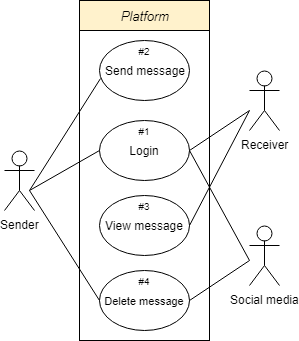
\includegraphics[width=0.50\linewidth]{Projectdoc/Assets/Illustrationer/simple-usecase.png}
                \end{figure}
            \end{block}
        \end{frame}
        
        \subsection{Krav}
        \begin{frame}{Kravsspecifikation}{Krav}
            \begin{block}{Krav til det fulde system}
                \begin{enumerate}
                    \footnotesize
                    \item \alert{Systemet skal kunne sende beskeder/indlæg}
                    \item \alert{Systemet skal kunne vise beskeder/indlæg}
                    \item \alert{Beskeder skal lagres på et socialt medie}
                    \item \alert{Lagrede beskeder skal være skjult via steganografi}
                    \item \alert{Systemet skal foretage kommunikationen anonymt}
                    \item \alert{Der må ikke forekomme indstillinger der påvirker brugernes sikkerhed}
                    \item Brugere skal kunne slette tidligere sendte beskeder
                    \item Beskeder skal kunne kædes i længere sammenhæng
                    \item 80\% af testbrugerne skal kunne navigere systemet uden yderligere instruktioner
                    \item Det skal være tydeligt for mindst 80\% af testbrugerne, at deres kommunikation er sikker
                    \item Systemet må ikke udelukkende sikres med steganografi
                    \item Systemet må ikke tage mere end 10 sekunder om at indlæse en indlægsoversigt
                \end{enumerate}
            \end{block}
        \end{frame}
    
    \section{System design}
    
        \subsection{Netværksstruktur}
        \begin{frame}{System design}{Netværksstruktur}
            \begin{block}{Central eller decentral løsning}
            
            \end{block}
        \end{frame}
        
        \subsection{}
        \begin{frame}{System design}{}
            \begin{block}{}
            
            \end{block}
        \end{frame}
        
        \subsection{Beskedkæder}
        \begin{frame}{System design}{Beskedkæder}
            
        \end{frame}
    
    \section{Præsentation af prototype}
        \subsection{Funktionalitet}
        \begin{frame}{Præsentation af prototype}{Funktionalitet}
            \begin{itemize}
                \item 
                %Hvad skal der ske.. step by step
            \end{itemize}
        \end{frame}
        \subsection{Mangler}
        \begin{frame}{Præsentation af prototype}{Mangler}
            \begin{itemize}
                \item 
                %Hvad fandt vi ud af der gav problemer eller ikke nåede at teste
            \end{itemize}
        \end{frame}
    
    \section{Process analyse}
        \subsection{Arbejdsgangen}
        \begin{frame}{Process analyse}{Arbejdsgangen}
            
        \end{frame}
        
        \subsection{Nye erfaringer}
        \begin{frame}{Process analyse}{Nye erfaringer}
            \begin{block}{Do's and Dont's}
                Do's
                \begin{itemize}
                    \item 
                \end{itemize}
                Dont's
                \begin{itemize}
                    \item 
                \end{itemize}
            \end{block}
        \end{frame}
        
        
        \subsection{Sammenholdet}
        \begin{frame}{Process analyse}{Sammenholdet}
            
        \end{frame}
    
    {\aauwavesbg
    \begin{frame}[plain,noframenumbering]
      \finalpage{Det var alt for den 25 øre!}
    \end{frame}}
\end{document}
